\documentclass[pdf]{beamer}
\usepackage[latin1]{inputenc}
\usepackage{multirow}
\usetheme{Antibes} %Warsaw
\usecolortheme{wolverine}


\begin{document}

\title[Sequence Assembly]{Sequence Assembly}
\subtitle{BCB 504: Applied Bioinformatics\\}
\author[Matt Settles]{Matt Settles}
\institute{University of Idaho\\ Bioinformatics and Computational Biology Program}
\date{\today}


%% Title page
\begin{frame}[plain]
  \titlepage
\end{frame}


%% Outline
\begin{frame}[plain] 
  \frametitle{Outline}
  \tableofcontents
\end{frame}

\section{Introduction}
\begin{frame}
  \frametitle{Assembly}
Shotgun Sequencing (Fred Sanger 1982) is the prevalent technique today
\begin{itemize}
\item Physically and randomly break the DNA into known sizes fragments.
\item DNA sequencer reads the DNA fragments.
\item Assembler reconstructs the original long sequence.
\end{itemize}
Assembly is challenging
\begin{itemize}
\item Data contains errors.
\item DNA has repetitive sections called repeats.
\item Gaps or un-sequenced fragments.
\item Lots of data, computationally difficult.
\end{itemize}
\end{frame}

\begin{frame}
\frametitle{Basic Approach - de novo assembly}
\begin{enumerate}
\item Sequence DNA to a specified depth.
\item Assemble reads into continuous sequence (aka contigs).
\item Order and orient contigs using additional information (aka scaffold).
\begin{itemize}
\item Paired end (or mate pair reads).
\item Optical mapping (high-resolution restriction maps)
\end{itemize}
\item Finish (gap closure, resequence low quality regions)
\end{enumerate}
\end{frame}

%
\section{Assembly Strategies}
\begin{frame}
\frametitle{Assembly Strategies}
\begin{itemize}
\item Greedy-extension (old school)
\item Overlap-layout-consensus (OLC) (small genomes)
\item De Bruijn graph (large genomes)
\end{itemize}
\end{frame}
%%%
\begin{frame}
\frametitle{Algorithms}
\begin{center}
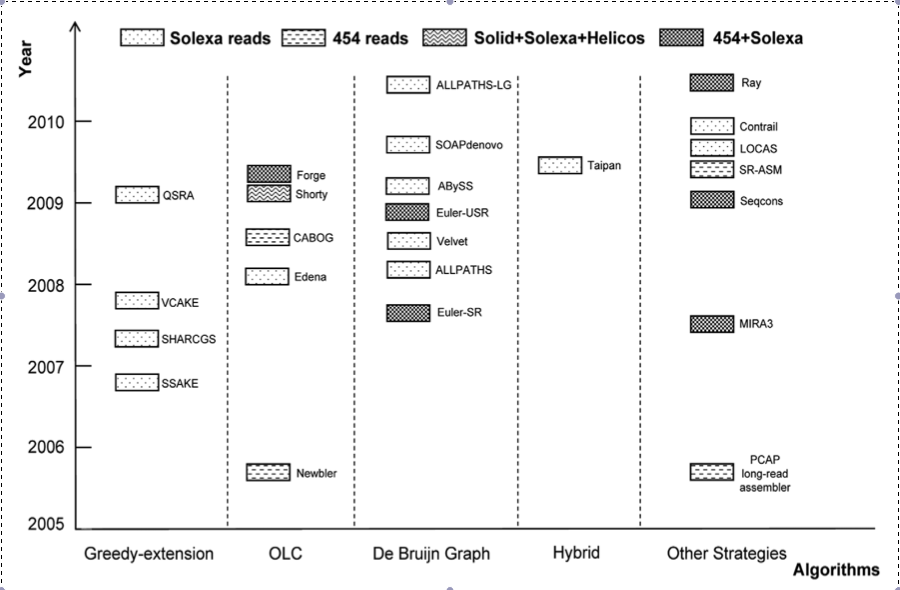
\includegraphics[scale=.32]{Figures/algorithms.png} 
\end{center}
\end{frame}

\section{Greedy-extension}
\begin{frame}
\frametitle{Greedy-extension}
Simple but effective strategy in which the assembler greedily joins together the reads that are the most similar to each other (largest overlap), as long as they do not contradict the already contructed assembly. 
\vspace{0.2in}
A major disadvantage of the simple greedy approach is that because local information is considered at each step and not the global relationship between reads, the assembler can be easily confused by complex repeats, leading to mis-assemblies.
\end{frame}

\begin{frame}
\frametitle{Greedy-extension (cont.)}
\begin{center}
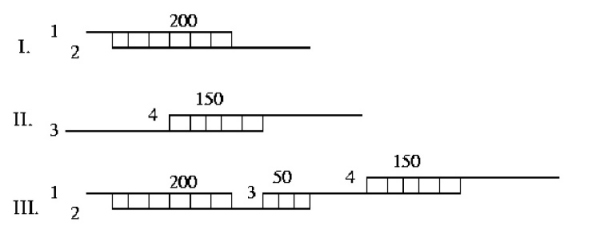
\includegraphics[scale=1]{Figures/greedy.jpg} 
\end{center}
\end{frame}

\section{Overlap-Layout-Consensus}

\begin{frame}[fragile]
\frametitle{Overlap-Layout-Consensus}
The assembler starts by identifying all paris of reads that overlap sufficiently (by some predetermined criteria) and then organizes this information into a graph containing a node for every read and an edge between any pair of reads that overlap each other. The graph structure allows the development of complex assembly algorithms that can take into account the global relationship between the reads.
\vspace{0.2in}
Largest concern of OLC assemblers is the computational complexity of the overlap computation.
\end{frame} 

\begin{frame}[fragile]
\frametitle{Overlap-Layout-Consensus}
\begin{verbatim}
To be or not to
    e or not to be, th
         not to be, that is the q
                 e, that is the question.
To be or not to be, that is the question.
\end{verbatim}
\end{frame}

\begin{frame}
\frametitle{Overlap-Layout-Consensus (overlap)}
\textbf{overlap}
find all the significant matches between pairs of reads\\
complexity of the order of N x N\\
remember all significant matches\\
Smarter solution:
\begin{small}
\begin{itemize}
\item Only n x coverage (e.g. 8) pairs are possible
\item Build a table of k-mers contained in sequences (single pass through the genome)
\item Generate the pairs from k-mer table (single pass through k-mer table)
\end{itemize}
\end{small}
\end{frame}


\begin{frame}
\frametitle{Overlap-Layout-Consensus (overlap)}
\begin{center}
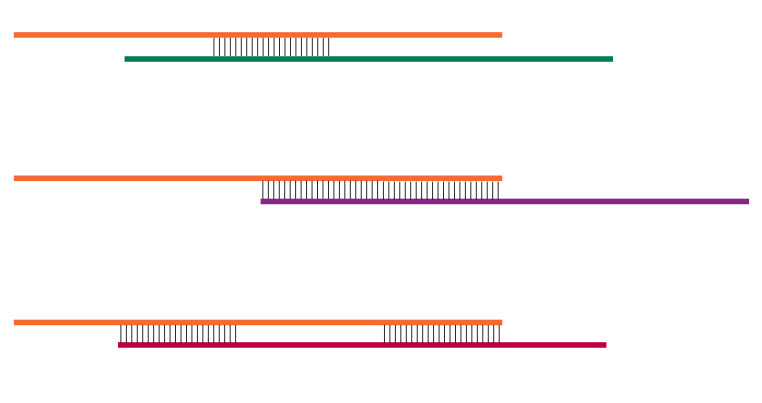
\includegraphics[scale=0.5]{Figures/overlap.png}
\end{center}
\end{frame}
 
\begin{frame}
\frametitle{Overlap-Layout-Consensus (layout)}
\textbf{layout}
parse the list of matches to satisfy simplest path through the list matching paired reads.\\
graph is simplified by removing redundant information.\\
Graph algorithms (Hamiltonian path,Eulerian path others) are then used to determine a layout (relative placement) of the reads along the genome
\end{frame}


\begin{frame}
\frametitle{Overlap-Layout-Consensus (layout)}
\begin{center}
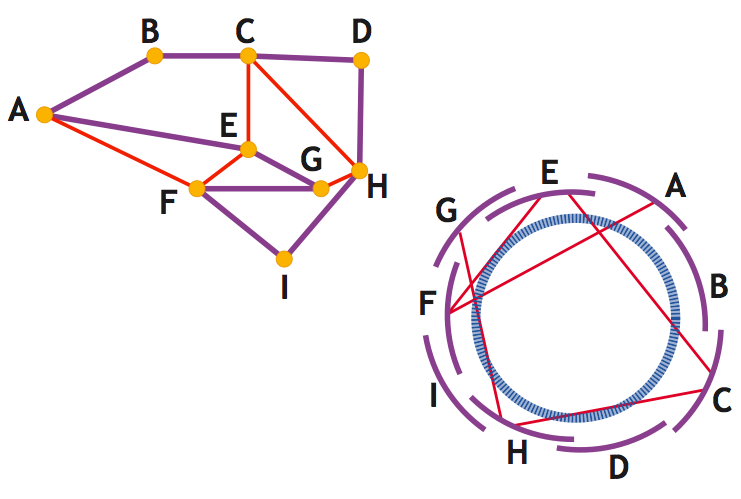
\includegraphics[scale=0.35]{Figures/layout.png}
\end{center}
\end{frame}

\begin{frame}
\frametitle{Overlap-Layout-Consensus (consensus)}
\textbf{consensus}
Derive a single consensus sequence for each set of contiguated reads (contig) following rules to deal with heterozygosity, errors and anomalies.\\
Builds an alignment of all the reads covering the genome and infers, as a consensus of the aligned reads, the original sequence of the genome being assembled.
\end{frame}

\section{De Bruijn Graph Assembler}
\begin{frame}
\frametitle{De Bruijn Graphs}
Assembling hundreds of millions of reads (and very short reads)\\
\vspace{0.2in}
\textbf{Problem with Overlap-Layout-Consensus}\\
The layout problem is formulated as the Shortest Superstring Problem, but the major difficulty is that there is no efficient algorithm for the solution of the layout problem.\\
\vspace{0.2in}
Heuristics are used to overcome this problem, but will often induce errors.
\vspace{0.1in}
Enter De Bruijn Assemblers
\end{frame}

\begin{frame}
\frametitle{De Bruijn Graphs}
De Bruijn graph assemblers model the relationship betwee exact substrings of length \textit{k} extracted from the input reads. Similarly to the OLC approach, the nodes in the graph represent \textit{k}-mers, and the edges indicate that the adjacent \textit{k}-mers overlap by exactly \textit{k}-1 letters. Whereas the reads themselves are not directly modelled in this paradigm (as they are in OLC), they are implicitely represented as paths through the de Bruijn graph. 
\vspace{0.1in}
Most de Bruijn assemblers us the read information to refine the graph structure and to remove graph patterns that are not consistant with the reads. Since the de Bruijn approach is based on exact matches, error correction approaches are crucial for achieving high quality assemblies.
\end{frame}

\begin{frame}
\frametitle{De Bruijn Graphs}
\begin{itemize}
\item split reads into k-mers
\begin{itemize}
\item k $<$ read length (usually $<<$ read length), but $>$ 19
\item K must also be odd
\end{itemize}
\item build De Bruijn graph of k-mers
\begin{itemize}
\item nodes are k-mers and edges indicate overlaps (reads can be split)
\end{itemize}
\item deconvolute graph to derive assembly
\begin{itemize}
\item the Eulerian cycle problem - visit every edge once (simpler to solve)
\end{itemize}
\end{itemize}

\end{frame}

\begin{frame}
\frametitle{De Bruijn Graphs}
\begin{center}
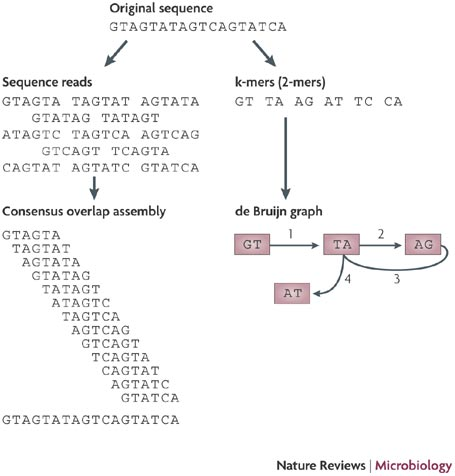
\includegraphics[scale=0.45]{Figures/smallEx.jpg} 
\end{center}
\end{frame}


\begin{frame}
\frametitle{De Bruijn Graphs}
In the de Bruijn graph, each node $N$ represents a series of overlapping k-mers. Adjacent k-mers overlap by k-1 nucleotides.\\
\vspace{0.2in}
The marginal information contained by a k-mer is its last nucleotide. The seuqence of those final nucleotides is called the sequences of the node ($s(N)$). Each node $N$ is attached to a twin node $N_c$ which represenet the reverse compliment of the k-mers. $N$ and $N_c$ for a BLOCK.\\
\vspace{0.2in}
BLOCKS are joined by ARCS.\\
The last k-mer of an arc's origin node overlaps with the first of its destination node.\\
Reads are mapped as "paths" traversing the graph.
\end{frame}

\begin{frame}
\frametitle{De Bruijn Graphs}
\begin{center}
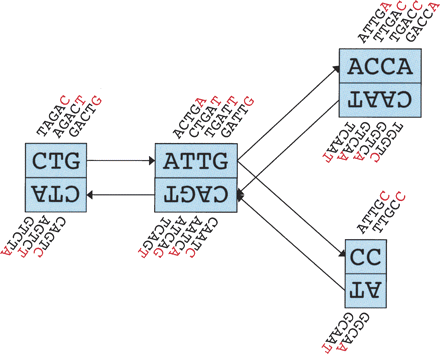
\includegraphics[scale=0.5]{Figures/velvet_blocks.png} 
\end{center}
\end{frame}

\begin{frame}
\frametitle{De Bruijn Graphs}
\textbf{Simplification}\\
After constructing the graph, it is generally possible to simplify it without any loss of information. Whenever a node $A$ has only one outgoing arc that points to another node $B$ that has only one ingoingarc, the nodes (and their twins) can be merged.
\end{frame}

\begin{frame}
\frametitle{De Bruijn Graphs}
\begin{center}
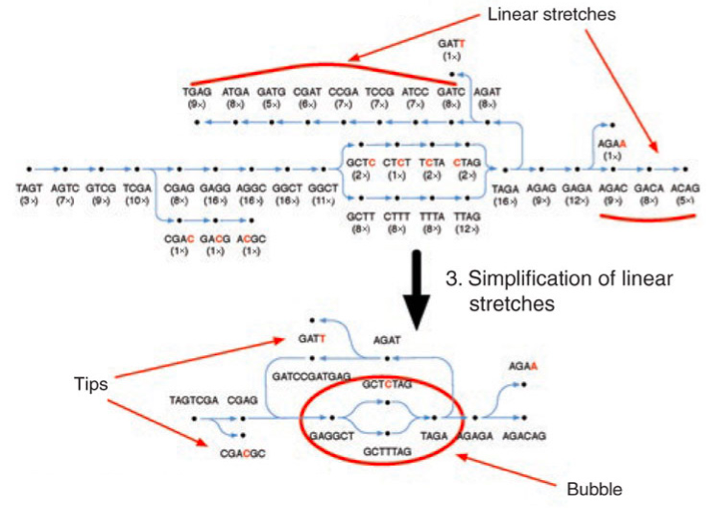
\includegraphics[scale=0.4]{Figures/simplification.png}
\end{center}
\end{frame}

\begin{frame}[allowframebreaks]
\frametitle{De Bruijn Graphs - error structures}
\textbf{Error removal}\\
Erroneous data create three types of structures:
\begin{itemize}
\item "tips" due to errors at the edges of reads.
\begin{itemize}
\item A "tip: is a chain of nodes that is disconnected at one end. Removing these tips is a straightforward task. Discarding this information results in only local effects and no connectivity is disrupted.
\end{itemize}
\item "bulges" or bubbles due to internal read errors or to nearby tips connecting.
\begin{itemize}
\item Two paths are redundant if they start and end at the same nodes and contain similar sequences.
\end{itemize}
\end{itemize}
\end{frame}

\begin{frame}
\frametitle{De Bruijn Graphs - error structures}
\textbf{Error removal (cont)}\\
\begin{itemize}
\item erroneous connections due to cloning errors or to distant merging tips.
\begin{itemize}
\item After the above corrections, genuine short nodes that cannot be simplified correspond to low-complexity sequences that are generally present multiple times in the genome. Their overall coverage is therefore proportionally higher than expected. This means that with a high probability, any low coverage node left after tip and bulge resolution is a chimeric connection, due to spurious overlaps, created by experimental errors.
\end{itemize}
\end{itemize}
\end{frame}

\begin{frame}
\frametitle{De Bruijn Graphs - error structures}
\begin{center}
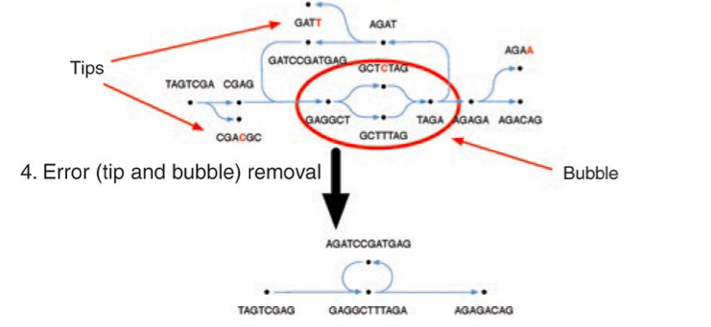
\includegraphics[scale=0.45]{Figures/error-removal.png} 
\end{center}
\end{frame}

\begin{frame}
\frametitle{De Bruijn Graphs - deconvolute graph}
\textbf{deconvolute graph to derive assembly\\ -the Eulerian cycle problem, find a path that visits every edge once}\\
\begin{center}
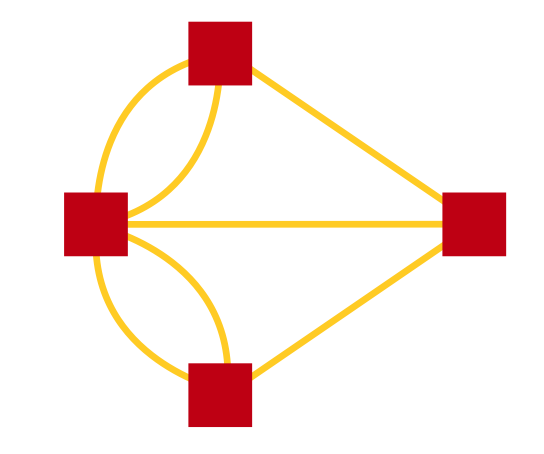
\includegraphics[scale=0.2]{Figures/eurler.png} 
\end{center}
tends to be exponential BUT can efficiently traverse the graph using the BEST theorem
\end{frame}

\begin{frame}
\frametitle{De Bruijn Graphs - deconvolute graph}
\begin{center}
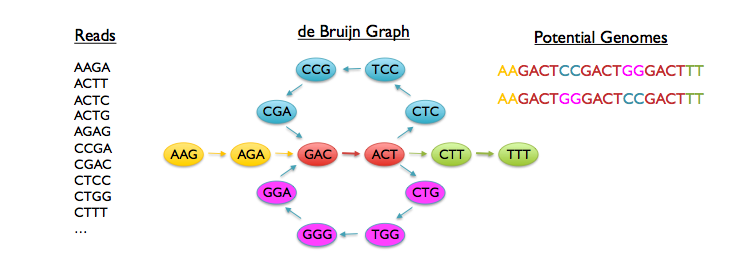
\includegraphics[scale=.45]{Figures/eulerreduce.png} 
\end{center}
De Bruijn graph assembly and traversal is compute intensive: Building a graph for the human genome from real data requires $>$ 3 billion nodes and $>$ 10 billion edges
\end{frame}

\section{Parameter Considerations}
\begin{frame}
\frametitle{Assembly Parameter Considerations}
\textbf{k-mer choice}\\
Longer k-mers bring you more specificity (i.e. less spurious overlaps) but lowers coverage, so there's a sweet spot to be found with time and experience.\\
\vspace{.1in}
Velvet suggests to think in terms of "k-mer coverage", i.e. how many times has  a k-mer been seen among the reads. The relation between k-mer coverage ($C_k$) and nucleotide coverage ($C$) is $C_k = C*(l-k+1)/L$, where $k$ is the k-mer length (hash length), and $L$ is the read length. \\
\vspace{.1in}
Velvet suggests that the k-mer coverage should be above 10 and If $C_k$ is above 30, you might be "wasting" coverage (20-30 is supposed to be ideal). k-mer choice is going to have the largest influence in the results, so its often best to try many.
\end{frame}

%\section{Output}
%\begin{frame}
%\frametitle{Cleaning reads}
%
%\end{frame}
%
%\section{Running an Assembly on the CRC}
%\begin{frame}
%\frametitle{Running an Assembly on the CRC}
%
%\end{frame}

\section{Resources}
\begin{frame}
\frametitle{Resources}
\begin{itemize}
\item http://seqanswers.com
\item http://seqanswers.com/wiki/SEQanswers
\end{itemize}
\end{frame}

\end{document}
